%\documentclass[handout]{beamer} % \pause disabled
\documentclass[t]{beamer} % \pause enabled
%%%%%%%%%%%%%%%%% Arya's
\usepackage{color,hyperref}
\hypersetup{colorlinks,breaklinks,linkcolor=darkblue,urlcolor=darkblue, anchorcolor=darkblue,citecolor=darkblue}
\usepackage{amsmath}
\usepackage{amsfonts}
\usepackage{amssymb}
\usepackage{mathtools}
\usepackage{enumerate}
\definecolor{darkgreen}{rgb}{0,0.55,0}
\definecolor{orange}{rgb}{1,0.55,0}
\definecolor{darkblue}{rgb}{0.0,0.0,0.5}
\def\Arya#1{{\textcolor{darkgreen}{Arya note: #1}}}

\newtheorem{Thm}{Theorem}


\newcommand{\dataset}{{\cal D}}
\newcommand{\fracpartial}[2]{\frac{\partial #1}{\partial  #2}}
\newcommand{\phibp}{\phi_{ \hspace{-0.025in}\scalebox{.45}{\text{ BP}}}}
\newcommand{\phics}{\phi_{ \hspace{-0.025in}\scalebox{.45}{\text{ CS}}}}
\newcommand{\lone}{$\ell_1$-norm }
%\def\lll{\mbox{\ell_1}}

%%%%%%%%%%%%%%%%% Anima Anandkumar's macros
\DeclareMathOperator{\tw}{tw}
\DeclareMathOperator{\local}{local}
\DeclareMathOperator{\range}{range}
\DeclareMathOperator{\Path}{Path}
\DeclareMathOperator{\Sg}{Sg}
\DeclareMathOperator{\spt}{SP}
\DeclareMathOperator{\avg}{avg}
\DeclareMathOperator{\nbd}{\mathcal{N}}
\DeclareMathOperator{\parent}{Pa}
\DeclareMathOperator{\Cq}{Cq}
\DeclareMathOperator{\TW}{TW}
\DeclareMathOperator{\approxML}{ApproxML}
\DeclareMathOperator{\Bethe}{Bethe}
\DeclareMathOperator{\TRW}{TRW}
\DeclareMathOperator{\conv}{Conv}
\DeclareMathOperator{\dir}{Dir}
\DeclareMathOperator{\mult}{Mult}
\DeclareMathOperator{\cat}{Cat}
\DeclareMathOperator{\crp}{CRP(\gamma)}
\DeclareMathOperator{\ncrp}{nCRP}
\DeclareMathOperator{\node}{node}
\DeclareMathOperator{\nodes}{nodes}
\DeclareMathOperator{\pr}{Pr}
\DeclareMathOperator{\dom}{\bf Dom}
\DeclareMathOperator{\lbp}{LBP}
\DeclareMathOperator{\Corr}{Corr}
\DeclareMathOperator{\hCorr}{\widehat{Corr}}
\DeclareMathOperator{\hSc}{\widehat{\mathcal{S}}}
\DeclareMathOperator{\tr}{Tr}
\DeclareMathOperator{\mst}{MST}
\DeclareMathOperator{\supp}{Supp}
\DeclareMathOperator{\dtv}{d_{TV}}
\DeclareMathOperator{\hdtv}{\hd_{TV}}
\DeclareMathOperator*{\argmin}{arg\,min}
\DeclareMathOperator*{\argmax}{arg\,max}
\DeclareMathOperator*{\esssup}{ess\,sup}
\DeclareMathOperator*{\essinf}{ess\,inf}
\DeclareMathOperator{\dist}{dist}
\DeclareMathOperator{\rank}{Rank}
\DeclareMathOperator{\Krank}{Rank_K}
\DeclareMathOperator{\Det}{Det}
\DeclareMathOperator{\poiss}{Poiss}
\DeclareMathOperator{\unif}{Unif} \DeclareMathOperator{\Deg}{Deg}
\def\simiid{{\overset{i.i.d.}{\sim}}}
\def\lcv{{\,\,\underset{cv}{\leq}\,\,}}
\def\gcv{{\,\,\underset{cv}{\geq}\,\,}}
\def\lcx{{\,\,\underset{cx}{\leq}\,\,}}
\def\gcx{{\,\,\underset{cx}{\geq}\,\,}}
\def\leqst{{\,\,\overset{st}{\leq}\,\,}}
\def\geqst{{\,\,\overset{st}{\geq}\,\,}}
\def\eqdist{{\,\,\overset{d}{=}\,\,}}
\def\geqrh{{\,\,\overset{rh}{\geq}\,\,}}
\def\geqlr{{\,\,\overset{lr}{\geq}\,\,}}
\def\eqlr{{\,\,\overset{lr}{=}\,\,}}
\def\comment{{\mbox{\bf Comment\_Anima: }}}
\def\tha{{\mbox{\tiny th}}}

\DeclareMathOperator{\Aug}{Aug}
\DeclareMathOperator{\watts}{Watts}
\DeclareMathOperator{\girth}{Girth}
\DeclareMathOperator{\PL}{PL}
\DeclareMathOperator{\LP}{LP}
\DeclareMathOperator{\ER}{ER}
\DeclareMathOperator{\reg}{Reg}
\DeclareMathOperator{\Var}{Var}
\DeclareMathOperator{\hSigma}{\widehat{\Sigma}}
\DeclareMathOperator{\Cov}{Cov}
\DeclareMathOperator{\Poiss}{Poiss}
\DeclareMathOperator{\Diag}{Diag}
\DeclareMathOperator{\Diam}{Diam}
\def\erf{\mbox{erf}}
\def\erfc{\mbox{erfc}}
\def\qfunc{\mbox{Q}}
%\def\myexp{\mbox{e}}
\def\snr{\mbox{{SNR}}}
\def\signum{\mbox{sgn}}
\def\Card{\mbox{Card}}
\DeclareMathOperator*{\plim}{plim}
\def\convd{\overset{d}\rightarrow}
\def\convp{\overset{p}\rightarrow}
\newcommand\indep{\protect\mathpalette{\protect\independenT}{\perp}}
\def\independenT#1#2{\mathrel{\rlap{$#1#2$}\mkern2mu{#1#2}}}
\def\pl{{\parallel}}
\DeclarePairedDelimiter\norm{\lVert}{\rVert}
\DeclarePairedDelimiter\nuclearnorm{\lVert}{\rVert_*}
\DeclarePairedDelimiter\onenorm{\lVert}{\rVert_1}
\DeclarePairedDelimiter\znorm{\lVert}{\rVert_0}
\def\rinfnorm{\rVert_{\infty}}
\DeclarePairedDelimiter\infnorm{\lVert}{\rinfnorm}
\def\lnorm{{\lvert\!\lvert\!\lvert}}
\def\rnorm{{\rvert\!\rvert\!\rvert}}
\DeclarePairedDelimiter\gennorm{\lnorm}{\rnorm}
 \DeclarePairedDelimiter\abs{\lvert}{\rvert}
 \DeclarePairedDelimiter\geninfnorm{\lnorm}{\rnorm_{\infty}}
 \DeclarePairedDelimiter\genonenorm{\lnorm}{\rnorm_{1}}
\DeclareMathOperator{\atanh}{atanh}
 \DeclareMathOperator{\sech}{sech}
 \def\0{{\bf 0}}

\DeclareMathOperator{\lea}{\overset{(a)}{\leq}}
\DeclareMathOperator{\leb}{\overset{(b)}{\leq}}
\DeclareMathOperator{\lec}{\overset{(c)}{\leq}}
\DeclareMathOperator{\led}{\overset{(d)}{\leq}}
\DeclareMathOperator{\lee}{\overset{(e)}{\leq}}

\DeclareMathOperator{\eqa}{\overset{(a)}{=}}
\DeclareMathOperator{\eqb}{\overset{(b)}{=}}
\DeclareMathOperator{\eqc}{\overset{(c)}{=}}
\DeclareMathOperator{\eqd}{\overset{(d)}{=}}
\DeclareMathOperator{\eqe}{\overset{(e)}{=}}

\DeclareMathOperator{\gea}{\overset{(a)}{\geq}}
\DeclareMathOperator{\geb}{\overset{(b)}{\geq}}
\DeclareMathOperator{\gec}{\overset{(c)}{\geq}}
\DeclareMathOperator{\ged}{\overset{(d)}{\geq}}
\DeclareMathOperator{\gee}{\overset{(e)}{\geq}}

\def\viz{{viz.,\ \/}}
\def\ie{{i.e.,\ \/}}
\def\eg{{e.g.,\ \/}}
\def\etc{{etc.  }}
\def\ifff{{iff  }}
\def\as{{a.s.  }}
\def\st{{s.t.  }}
\def\wpone{{w.p.}\,1\,\,}
\def\wpp{{w.p.p.}\,\,}
\def\for{\,\,\mbox{for}\quad}
\def\ifmbox{\,\,\mbox{if}\quad}
\def\nn{\nonumber}
%\def\qed{\hfill$\Box$}

\def\qed{\hfill\hbox{${\vcenter{\vbox{
    \hrule height 0.4pt\hbox{\vrule width 0.4pt height 6pt
    \kern5pt\vrule width 0.4pt}\hrule height 0.4pt}}}$}}
\def\complx{\mathbb{C}}

%%%%%%%%%%%%%%%%%%%%%%%%%%%%%%%%%%%%%%%%%%%%%%%%%%%%%%%%%%%%% Color

\def\tcr{\textcolor{red}}
\def\tcb{\textcolor{blue}}
\def\tcg{\textcolor{green}}
\def\tcw{\textcolor{white}}
\def\tcm{\textcolor{magenta}}
\def\tccyan{\textcolor{cyan}}
\def\tcv{\textcolor{violet}}
\definecolor{myred}{rgb}{0.3,0.0,0.7}
\definecolor{dkg}{rgb}{0.1,0.7,0.2}
\definecolor{dkb}{rgb}{0.0,0.2,0.8}

\def\tcdkb{\textcolor{dkb}}
\def\tcdkg{\textcolor{dkg}}


%%%%%%%%%%%%%%%%%%%%%%%%%%%%%%%%%%%%%%%%%%%%%%%%%%%%%%%%%%%%%
\newcommand{\Amsc}{\mathscr{A}}
\newcommand{\Cmsc}{\mathscr{C}}
\newcommand{\Dmsc}{\mathscr{D}}
\newcommand{\Emsc}{\mathscr{E}}
\newcommand{\Fmsc}{\mathscr{F}}
\newcommand{\Gmsc}{\mathscr{G}}
\newcommand{\Hmsc}{\mathscr{H}}
\newcommand{\Kmsc}{\mathscr{K}}
\newcommand{\Nmsc}{\mathscr{N}}
\newcommand{\Pmsc}{\mathscr{P}}
\newcommand{\Qmsc}{\mathscr{Q}}
\newcommand{\Rmsc}{\mathscr{R}}
\newcommand{\Smsc}{\mathscr{S}}
\newcommand{\Tmsc}{\mathscr{T}}
\newcommand{\Umsc}{\mathscr{U}}
\newcommand{\Xmsc}{\mathscr{X}}
\newcommand{\Ymsc}{\mathscr{Y}}

%%%%%%%%%%%%%%%%%%%%%%%%%%%%%%%%%%%%%%%%%%%%%%%%%%%%%%%%%%%%% Hat
\def\ha{\widehat{a}}
\def\hb{\widehat{b}}
\def\hc{\widehat{c}}
\def\hd{\widehat{d}}
\def\he{\widehat{e}}
\def\hf{\widehat{f}}
\def\hg{\widehat{g}}
\def\hh{\widehat{h}}
\def\hi{\widehat{i}}
\def\hj{\widehat{j}}
\def\hk{\widehat{k}}
\def\hl{\widehat{l}}
\def\hm{\widehat{m}}
\def\hn{\widehat{n}}
\def\ho{\widehat{o}}
\def\hp{\widehat{p}}
\def\hq{\widehat{q}}
\def\hr{\widehat{r}}
\def\hs{\widehat{s}}
\def\hatt{\widehat{t}}
\def\hu{\widehat{u}}
\def\hv{\widehat{v}}
\def\hw{\widehat{w}}
\def\hx{\widehat{x}}
\def\hy{\widehat{y}}
\def\hz{\widehat{z}}

\def\hA{\widehat{A}}
\def\hB{\widehat{B}}
\def\hC{\widehat{C}}
\def\hD{\widehat{D}}
\def\hE{\widehat{E}}
\def\hF{\widehat{F}}
\def\hG{\widehat{G}}
\def\hH{\widehat{H}}
\def\hI{\widehat{I}}
\def\hJ{\widehat{J}}
\def\hK{\widehat{K}}
\def\hL{\widehat{L}}
\def\hM{\widehat{M}}
\def\hN{\widehat{N}}
\def\hO{\widehat{O}}
\def\hP{\widehat{P}}
\def\hQ{\widehat{Q}}
\def\hR{\widehat{R}}
\def\hS{\widehat{S}}
\def\hT{\widehat{T}}
\def\hU{\widehat{U}}
\def\hV{\widehat{V}}
\def\hW{\widehat{W}}
\def\hX{\widehat{X}}
\def\hY{\widehat{Y}}
\def\hZ{\widehat{Z}}
\def\hlambda{\widehat{\lambda}}
\def\hpi{\widehat{\pi}}
\def\hnu{\widehat{\nu}}
\def\hbd{\widehat{\mathbf{d}}}
\def\bLambda{\mathbf{\Lambda}}

%%%%%%%%%%%%%%%%%%%%%%%%%%%%%%%%%%%%%%%%%%%%%%%%%%%%%%%%%%%%% Bold
\def\bfnu{{\boldsymbol {\nu}}}
\def\bfzero{{\mathbf{0}}}
\def\bfone{{\mathbf{1}}}
\def\bfa{{\mathbf a}}
\def\bfb{{\mathbf b}}
\def\bfc{{\mathbf c}}
\def\bfd{{\mathbf d}}
\def\bfe{{\mathbf e}}
\def\bff{{\mathbf f}}
\def\bfg{{\mathbf g}}
\def\bfh{{\mathbf h}}
\def\bfi{{\mathbf i}}
\def\bfj{{\mathbf j}}
\def\bfk{{\mathbf k}}
\def\bfl{{\mathbf l}}
\def\bfm{{\mathbf m}}
\def\bfn{{\mathbf n}}
\def\bfo{{\mathbf o}}
\def\bfp{{\mathbf p}}
\def\bfq{{\mathbf q}}
\def\bfr{{\mathbf r}}
\def\bfs{{\mathbf s}}
\def\bft{{\mathbf t}}
\def\bfu{{\mathbf u}}
\def\bfv{{\mathbf v}}
\def\bfw{{\mathbf w}}
\def\bfx{{\mathbf x}}
\def\bfy{{\mathbf y}}
\def\bfz{{\mathbf z}}

\def\bfA{{\mathbf A}}
\def\bfB{{\mathbf B}}
\def\bfC{{\mathbf C}}
\def\bfD{{\mathbf D}}
\def\bfE{{\mathbf E}}
\def\bfF{{\mathbf F}}
\def\bfG{{\mathbf G}}
\def\bfH{{\mathbf H}}
\def\bfI{{\mathbf I}}
\def\bfJ{{\mathbf J}}
\def\bfK{{\mathbf K}}
\def\bfL{{\mathbf L}}
\def\bfM{{\mathbf M}}
\def\bfN{{\mathbf N}}
\def\bfO{{\mathbf O}}
\def\bfP{{\mathbf P}}
\def\bfQ{{\mathbf Q}}
\def\bfR{{\mathbf R}}
\def\bfS{{\mathbf S}}
\def\bfT{{\mathbf T}}
\def\bfU{{\mathbf U}}
\def\bfV{{\mathbf V}}
\def\bfW{{\mathbf W}}
\def\bfX{{\mathbf X}}
\def\bfY{{\mathbf Y}}
\def\bfZ{{\mathbf Z}}


%%%%%%%%%%%%%%%%%%%%%%%%%%%%%%%%%%%%%%%%%%%%%%%%%%%%%%%%%%%%% Bold Symbols
\def\alphabf{\hbox{\boldmath$\alpha$\unboldmath}}
\def\betabf{\hbox{\boldmath$\beta$\unboldmath}}
\def\gammabf{\hbox{\boldmath$\gamma$\unboldmath}}
\def\deltabf{\hbox{\boldmath$\delta$\unboldmath}}
\def\epsilonbf{\hbox{\boldmath$\epsilon$\unboldmath}}
\def\zetabf{\hbox{\boldmath$\zeta$\unboldmath}}
\def\etabf{\hbox{\boldmath$\eta$\unboldmath}}
\def\iotabf{\hbox{\boldmath$\iota$\unboldmath}}
\def\kappabf{\hbox{\boldmath$\kappa$\unboldmath}}
\def\lambdabf{\hbox{\boldmath$\lambda$\unboldmath}}
\def\mubf{\hbox{\boldmath$\mu$\unboldmath}}
\def\nubf{\hbox{\boldmath$\nu$\unboldmath}}
\def\xibf{\hbox{\boldmath$\xi$\unboldmath}}
\def\pibf{\hbox{\boldmath$\pi$\unboldmath}}
\def\rhobf{\hbox{\boldmath$\rho$\unboldmath}}
\def\sigmabf{\hbox{\boldmath$\sigma$\unboldmath}}
\def\taubf{\hbox{\boldmath$\tau$\unboldmath}}
\def\upsilonbf{\hbox{\boldmath$\upsilon$\unboldmath}}
\def\phibf{\hbox{\boldmath$\phi$\unboldmath}}
\def\chibf{\hbox{\boldmath$\chi$\unboldmath}}
\def\psibf{\hbox{\boldmath$\psi$\unboldmath}}
\def\omegabf{\hbox{\boldmath$\omega$\unboldmath}}
\def\inftybf{\hbox{\boldmath$\infty$\unboldmath}}
\def\hSigmabf{\hbox{$\widehat{\bf \Sigma}$}}
\def\Sigmabf{\hbox{$\bf \Sigma$}}
\def\Upsilonbf{\hbox{$\bf \Upsilon$}}
\def\Omegabf{\hbox{$\bf \Omega$}}
\def\Deltabf{\hbox{$\bf \Delta$}}
\def\Gammabf{\hbox{$\bf \Gamma$}}
\def\Thetabf{\hbox{$\bf \Theta$}}
\def\Lambdabf{\mbox{$ \bf \Lambda $}}
\def\Xibf{\hbox{\bf$\Xi$}}
\def\Pibf{{\bf \Pi}}
\def\thetabf{{\mbox{\boldmath$\theta$\unboldmath}}}
\def\Upsilonbf{\hbox{\boldmath$\Upsilon$\unboldmath}}
\newcommand{\Phibf}{\mbox{${\bf \Phi}$}}
\newcommand{\Psibf}{\mbox{${\bf \Psi}$}}
\def\olambda{\mathfrak{o}(\lambda)}
\def\complex{\mathfrak{C}}

%%%%%%%%%%%%%%%%%%%%%%%%%%%%%%%%%%%%%%%%%%%%%%%%%%%%%%%%%%%%% Bar
\def\brzero{{\overline{{0}}}}
\def\brone{{\overline{{1}}}}
\def\bra{{\overline{a}}}
\def\brb{{\overline{b}}}
\def\brc{{\overline{c}}}
\def\brd{{\overline{d}}}
\def\bre{{\overline{e}}}
\def\brf{{\overline{f}}}
\def\brg{{\overline{g}}}
\def\brh{{\overline{h}}}
\def\bri{{\overline{i}}}
\def\brj{{\overline{j}}}
\def\brk{{\overline{k}}}
\def\brl{{\overline{l}}}
\def\brm{{\overline{m}}}
\def\brn{{\overline{n}}}
\def\bro{{\overline{o}}}
\def\brp{{\overline{p}}}
\def\brq{{\overline{q}}}
\def\brr{{\overline{r}}}
\def\brs{{\overline{s}}}
\def\brt{{\overline{t}}}
\def\bru{{\overline{u}}}
\def\brv{{\overline{v}}}
\def\brw{{\overline{w}}}
\def\brx{{\overline{x}}}
\def\bry{{\overline{y}}}
\def\brz{{\overline{z}}}

\def\brA{{\overline{A}}}
\def\brB{{\overline{B}}}
\def\brC{{\overline{C}}}
\def\brD{{\overline{D}}}
\def\brE{{\overline{E}}}
\def\brF{{\overline{F}}}
\def\brG{{\overline{G}}}
\def\brH{{\overline{H}}}
\def\brI{{\overline{I}}}
\def\brJ{{\overline{J}}}
\def\brK{{\overline{K}}}
\def\brL{{\overline{L}}}
\def\brM{{\overline{M}}}
\def\brN{{\overline{N}}}
\def\brO{{\overline{O}}}
\def\brP{{\overline{P}}}
\def\brQ{{\overline{Q}}}
\def\brR{{\overline{R}}}
\def\brS{{\overline{S}}}
\def\brT{{\overline{T}}}
\def\brU{{\overline{U}}}
\def\brV{{\overline{V}}}
\def\brW{{\overline{W}}}
\def\brX{{\overline{X}}}
\def\brY{{\overline{Y}}}
\def\beZ{{\overline{Z}}}


%%%%%%%%%%%%%%%%%%%%%%%%%%%%%%%%%%%%%%%%%%%%%%%%%%%%%%%%%%%%% Bar Bold 
\def\bbfzero{{\overline{\mathbf{0}}}}
\def\bbfone{{\overline{\mathbf{1}}}}
\def\bbfa{{\overline{\mathbf a}}}
\def\bbfb{{\overline{\mathbf b}}}
\def\bbfc{{\overline{\mathbf c}}}
\def\bbfd{{\overline{\mathbf d}}}
\def\bbfe{{\overline{\mathbf e}}}
\def\bbff{{\overline{\mathbf f}}}
\def\bbfg{{\overline{\mathbf g}}}
\def\bbfh{{\overline{\mathbf h}}}
\def\bbfi{{\overline{\mathbf i}}}
\def\bbfj{{\overline{\mathbf j}}}
\def\bbfk{{\overline{\mathbf k}}}
\def\bbfl{{\overline{\mathbf l}}}
\def\bbfm{{\overline{\mathbf m}}}
\def\bbfn{{\overline{\mathbf n}}}
\def\bbfo{{\overline{\mathbf o}}}
\def\bbfp{{\overline{\mathbf p}}}
\def\bbfq{{\overline{\mathbf q}}}
\def\bbfr{{\overline{\mathbf r}}}
\def\bbfs{{\overline{\mathbf s}}}
\def\bbft{{\overline{\mathbf t}}}
\def\bbfu{{\overline{\mathbf u}}}
\def\bbfv{{\overline{\mathbf v}}}
\def\bbfw{{\overline{\mathbf w}}}
\def\bbfx{{\overline{\mathbf x}}}
\def\bbfy{{\overline{\mathbf y}}}
\def\bbfz{{\overline{\mathbf z}}}

\def\bbfA{{\overline{\mathbf A}}}
\def\bbfB{{\overline{\mathbf B}}}
\def\bbfC{{\overline{\mathbf{C}}}}
\def\bbfD{{\overline{\mathbf D}}}
\def\bbfE{{\overline{\mathbf E}}}
\def\bbfF{{\overline{\mathbf F}}}
\def\bbfG{{\overline{\mathbf G}}}
\def\bbfH{{\overline{\mathbf H}}}
\def\bbfI{{\overline{\mathbf I}}}
\def\bbfJ{{\overline{\mathbf J}}}
\def\bbfK{{\overline{\mathbf K}}}
\def\bbfL{{\overline{\mathbf L}}}
\def\bbfM{{\overline{\mathbf M}}}
\def\bbfN{{\overline{\mathbf N}}}
\def\bbfO{{\overline{\mathbf O}}}
\def\bbfP{{\overline{\mathbf P}}}
\def\bbfQ{{\overline{\mathbf Q}}}
\def\bbfR{{\overline{\mathbf R}}}
\def\bbfS{{\overline{\mathbf S}}}
\def\bbfT{{\overline{\mathbf T}}}
\def\bbfU{{\overline{\mathbf U}}}
\def\bbfV{{\overline{\mathbf V}}}
\def\bbfW{{\overline{\mathbf W}}}
\def\bbfX{{\overline{\mathbf X}}}
\def\bbfY{{\overline{\mathbf Y}}}
\def\bbfZ{{\overline{\mathbf Z}}}

%%%%%%%%%%%%%%%%%%%%%%%%%%%%%%%%%%%%%%%%%%%%%%%%%%%%%%%%%%%%% Calligraphic
\def\Ac{{\cal A}}
\def\Bc{{\cal B}}
\def\Cc{{\cal C}}
\def\Dc{{\cal D}}
\def\Ec{{\cal E}}
\def\Fc{{\cal F}}
\def\Gc{{\cal G}}
\def\Hc{{\cal H}}
\def\Ic{{\cal I}}
\def\Jc{{\cal J}}
\def\Kc{{\cal K}}
\def\Lc{{\cal L}}
\def\Mc{{\cal M}}
\def\Nc{{\cal N}}
\def\Oc{{\cal O}}
\def\Pc{{\cal P}}
\def\Qc{{\cal Q}}
\def\Rc{{\cal R}}
\def\Sc{{\cal S}}
\def\Tc{{\cal T}}
\def\Uc{{\cal U}}
\def\Vc{{\cal V}}
\def\Wc{{\cal W}}
\def\Xc{{\cal X}}
\def\Yc{{\cal Y}}
\def\Zc{{\cal Z}}


%%%%%%%%%%%%%%%%%%%%%%%%%%%%%%%%%%%%%%%%%%%%%%%%%%%%%%%%%%%%% Mathbb

\def\Abb{{\mathbb A}}
\def\BBb{{\mathbb B}}% different
\def\Cbb{{\mathbb C}}
\def\Dbb{{\mathbb D}}
\def\Ebb{{\mathbb E}}
\def\Fbb{{\mathbb F}}
\def\Gbb{{\mathbb G}}
\def\Hbb{{\mathbb H}}
\def\Ibb{{\mathbb I}}
\def\Jbb{{\mathbb J}}
\def\Kbb{{\mathbb K}}
\def\Lbb{{\mathbb L}}
\def\Mbb{{\mathbb M}}
\def\Nbb{{\mathbb N}}
\def\Obb{{\mathbb O}}
\def\Pbb{{\mathbb P}}
\def\Qbb{{\mathbb Q}}
\def\Rbb{{\mathbb R}}
\def\Sbb{{\mathbb S}}
\def\Tbb{{\mathbb T}}
\def\Ubb{{\mathbb U}}
\def\Vbb{{\mathbb V}}
\def\Wbb{{\mathbb W}}
\def\Xbb{{\mathbb X}}
\def\Ybb{{\mathbb Y}}
\def\Zbb{{\mathbb Z}}

%%%%%%%%%%%%%%%%%%%%%%%%%%%%%%%%%%%%%%%%%%%%%%%%%%%%%%%%%%%%% Command Abbreviations
%\newcommand{\bprfof}{\begin{proof_of}}
%\newcommand{\eprfof}{\end{proof_of}}
\newcommand{\bprf}{\begin{proof}}
\newcommand{\eprf}{\end{proof}}
%\newcommand{\bp}{\begin{psfrags}}
%\newcommand{\ep}{\end{psfrags}}
%\newcommand{\bl}{\begin{lemma}}
%\newcommand{\el}{\end{lemma}}
\newcommand{\bt}{\begin{theorem}}
\newcommand{\et}{\end{theorem}}
%\newcommand{\bc}{\begin{center}}
%\newcommand{\ec}{\end{center}}
%\newcommand{\bi}{\begin{itemize}}
%\newcommand{\ei}{\end{itemize}}
%\newcommand{\ben}{\begin{enumerate}}
%\newcommand{\een}{\end{enumerate}}
%\newcommand{\bd}{\begin{definition}}
%\newcommand{\ed}{\end{definition}}
\def\beq{\begin{equation}\begin{aligned}}
\def\eeq{\end{aligned}\end{equation}\noindent}
\def\beqq{\begin{equation*}\begin{aligned}}
\def\eeqq{\end{aligned}\end{equation*}\noindent}
\def\beqn{\begin{eqnarray}}
\def\eeqn{\end{eqnarray} \noindent}
%\def\beqnn{  \begin{eqnarray*}}
%\def\eeqnn{\end{eqnarray*}  \noindent}
%\def\bcase{  \begin{numcases}}
%\def\ecase{\end{numcases}   \noindent}
%\def\bsbcase{  \begin{subnumcases}}
%\def\esbcase{\end{subnumcases}   \noindent}
%
%\def\endproof{\hfill\blacksquare}
%\def\defeq{{:=}}%{{\stackrel{\Delta}{=}}}
%
%

\usepackage{datetime}
\def\vecbold#1{{\boldsymbol#1}}

\newdateformat{monthyeardate}{%
  \monthname[\THEMONTH], \THEYEAR}

%\usepackage[linesnumbered,ruled]{algorithm2e}
\usetheme{Madrid}
\setbeamertemplate{footline}
{
  \leavevmode%
  \hbox{%
  \begin{beamercolorbox}[wd=.333333\paperwidth,ht=2.25ex,dp=1ex,center]{author in head/foot}%
    \usebeamerfont{author in head/foot}\insertshortauthor
  \end{beamercolorbox}%
  \begin{beamercolorbox}[wd=.333333\paperwidth,ht=2.25ex,dp=1ex,center]{title in head/foot}%
    \usebeamerfont{title in head/foot}\insertshorttitle
  \end{beamercolorbox}%
  \begin{beamercolorbox}[wd=.333333\paperwidth,ht=2.25ex,dp=1ex,right]{date in head/foot}%
    \usebeamerfont{date in head/foot}\insertshortdate{}\hspace*{2em}
    \insertframenumber{} / \inserttotalframenumber\hspace*{2ex} 
  \end{beamercolorbox}}%
  \vskip0pt%
}
\def\dHAF{\text{-HAF}}
\makeatother
\title{Genomic Time-Series Data Analysis}
\subtitle{}
\author[Arya Iranmehr]
{%
  \texorpdfstring{
      \centering
      Arya Iranmehr\\
      \href{mailto:airanmehr@ucsd.edu}{airanmehr@ucsd.edu}
  }
  {Arya Iranmehr}
}
%\email{}
\institute{
Bafna Lab\\
University of California, San Diego}
\date{
\monthyeardate\today}
\subject{Optimization}
\usefonttheme{serif} % default family is serif
%\AtBeginSection[]
%  {
%     \begin{frame}<beamer>
%     \frametitle{Agenda}
%     \tableofcontents[currentsection,currentsubsection]
%     \end{frame}
%  }
%\AtBeginSubsection[]
%{
%  \begin{frame}<beamer>{Outline}
%    \tableofcontents[currentsection,currentsubsection]
%  \end{frame}
%}

\begin{document}
\begin{frame}
  \titlepage
\end{frame}




\begin{frame}
Experimental Evolution
\begin{figure}
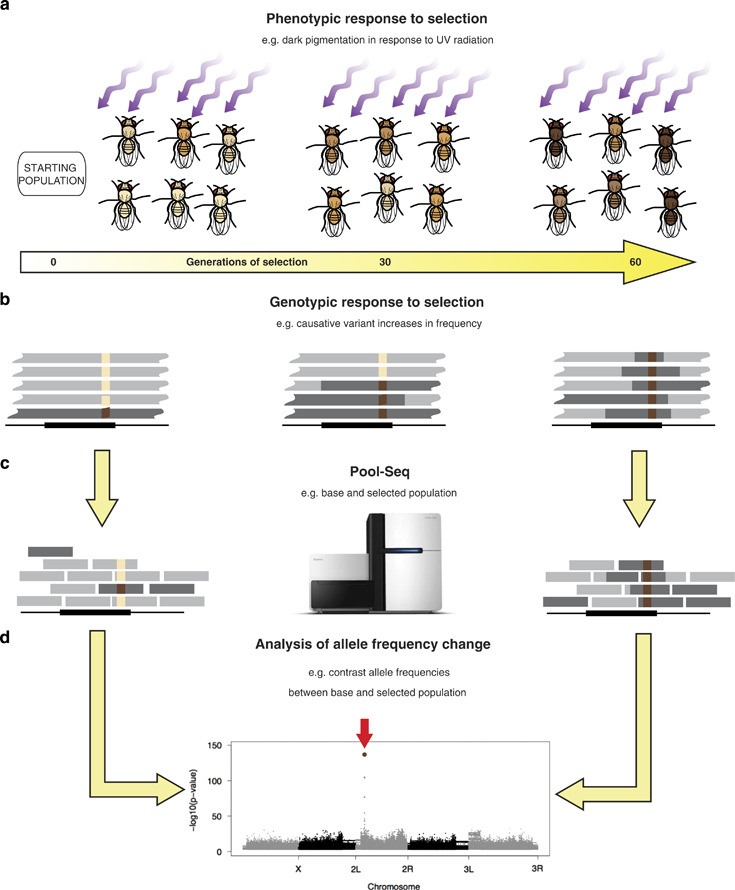
\includegraphics[trim={0 2.1in 0 0},clip, scale=0.6]{eg.jpg} 
\end{figure}
\end{frame}
\begin{frame}{Simulations}
\begin{enumerate}[(i)]
\item For each simulation, population of $F=200$ founder lines is created in  \texttt{msms} program with parameters 
\begin{itemize}
\item Length of genome $L=10^6$Kbp.
\item Population size $N_e=10^6$.
\item Recombination rate $r=2\times10^{-8}$.
\item Mutation rate $\mu=10^{-9}$ which give $\theta = 200$ and $m\approx 1200$ .
\end{itemize}

\item Using $F=200$ founder lines a population of $N=1000$ diploid homozygote individuals are created.
\item Using \texttt{SimuPop}, the initial population is forward simulated for 10 replicates and AF is recorded every 10 generation for a complete hard sweep. 
\item I.e., a site with minimum allele frequency of $1/F$ is always under selection.
\item for each $s=\{0.1, 0.05, 0.02, 0.01, 0\}$ 100 simulations are done.
\end{enumerate}
\end{frame}

\begin{frame}{Biological Goals}
\begin{itemize}
\item Given the genome time series data (allele frequencies) we are interested in
\begin{enumerate}[I]
\item Detecting selection 
\item Locating selection
\begin{enumerate}[(i)]
 \item Identify gene under selection
 \item Identify the mutation 
\end{enumerate}
\item Estimating model parameters
\end{enumerate}
\item  problems I and II are easier, and can be addressed using model-free methods such as Tajima's D.
\end{itemize}
\end{frame}

\begin{frame}{History Detecting and locating Selection}
\begin{itemize}
\item Traditionally, detecting/locating selection is done by analysing Allele Spectrum Frequency (AFS) from a window (50Kbp here).
\item different linear combinations of AFS vector gives different tests of selection.
\item to put it in context, Tajima's D, FayWu's H and SFSelect are multi-locus, model-free methods for detecting and locating selection which use a \emphr{ single snapshot} of data.
\item However, we extend these methods to times-series framework, just by summing all test statistics through time.
\end{itemize}
\end{frame}


\begin{frame}{Questions}
\begin{enumerate}[(i)]
\item Are multi-locus methods better than single locus ones?
\item Are time-series methods outperform single-snapshot methods?
\item Are model-based approaches (likelihood based methods such as GP) better than classical \emphr{model-free} statistical-tests for detecting selection?
\item When detecting and locating selection is trival and when is not?
\item How does the initial frequency of the carrier affect the performance?
\end{enumerate}


\end{frame}

\begin{frame}{Hard Sweep}
\begin{itemize}
\item With this setting around a quarter of sites are at MAF at time 0.
\item We will consider hard-sweep, i.e., site under selection frequency=$1/F=1/Ne=0.005$=MAF. 
\item if we pick a site randomly with high prob, it'll be low freq.
\end{itemize}
\hspace{-0in}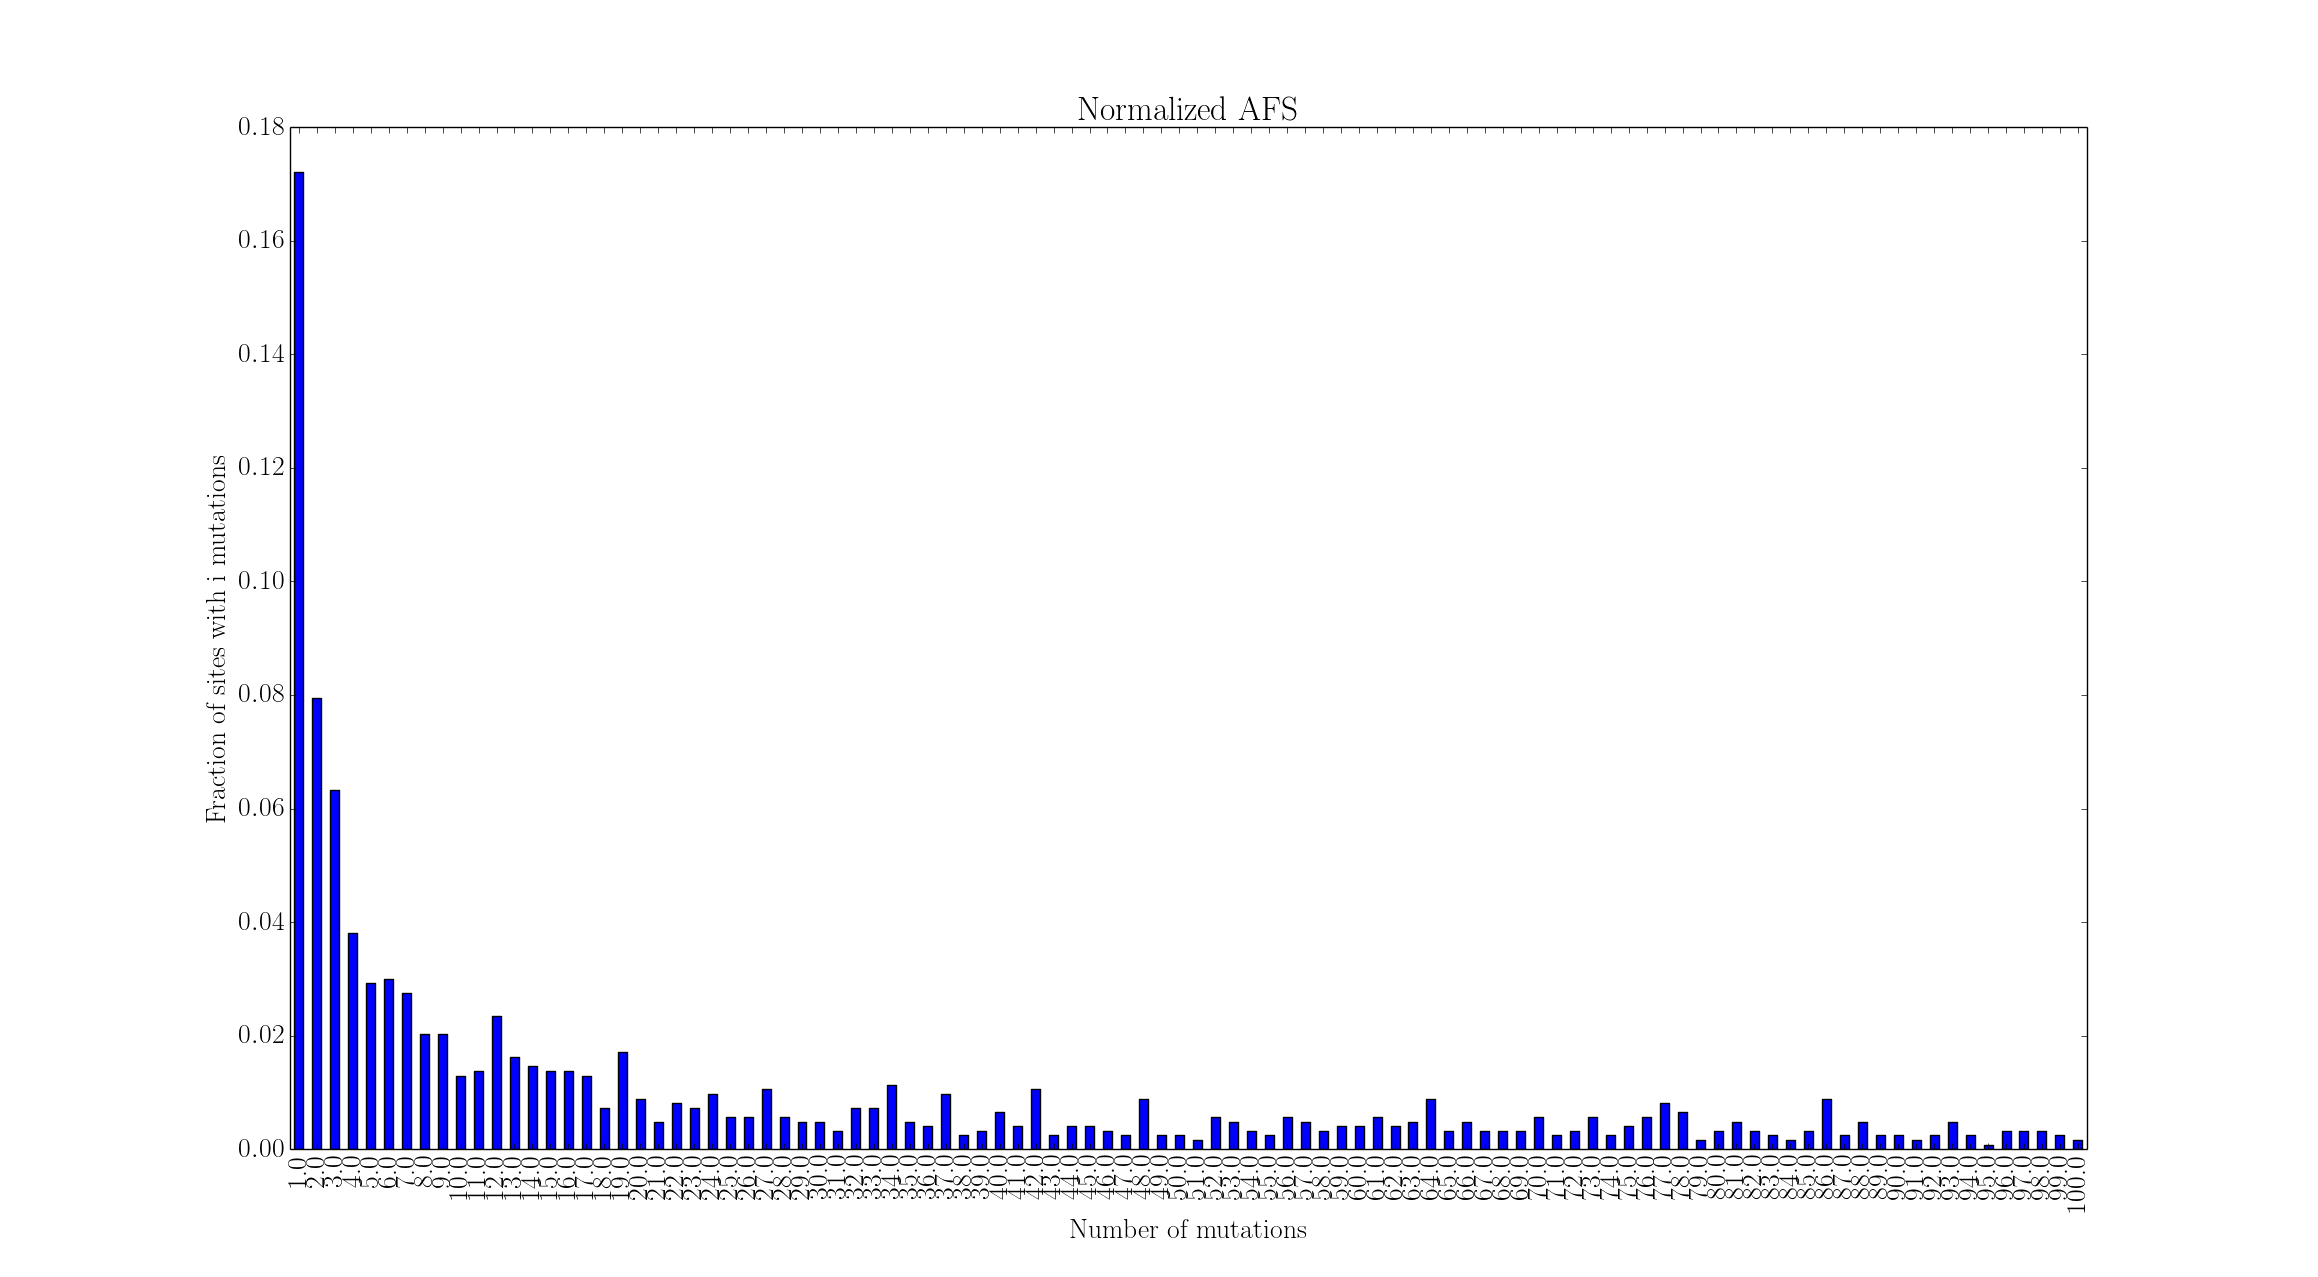
\includegraphics[scale=0.17]{AFS}
\end{frame}

\begin{frame}{Single Locus Logistic Model: Carrier Frequency}
Dynamics of sweep extremely depend on $s$ as well as initial carrier frequency.Sampling times are very important prediction performance!

\begin{figure}
\centering
\hspace{-0in}\includegraphics[trim={2in 0.5in 1.5in 0in},clip,page=2,width=0.5\textwidth]{sigmoidSoft}
\hspace{-0in}\includegraphics[trim={2in 0.5in 1.9in 0in},clip,page=2,width=0.5\textwidth]{sigmoidHard}
\end{figure}
{\tiny
\begin{enumerate}
\item Left) Terhorst et al. considered soft sweep. The time-window which  they sampled is shaded. 
\item Right) With the same sampling scheme, it is difficult to make predictions base on observations under 50 generations.
\end{enumerate}
}
\end{frame}

\begin{frame}{A Naive Single Locus Model}
\begin{itemize}
\item Roughly, just divide your last and first observation, it gives you a number, which can be regarded as a \emphr{predictor} for detecting selection. I.e., larger values of the predictor imply evidence of selection.
\item Using start and end AF at a site, we can solve the logistic equation to get an estimate of $s$ for that site.
\end{itemize}

\end{frame}

\begin{frame}{Multi-Locus Methods}
\begin{itemize}
\item In hard sweep, site under selection has perfect LD with all the other sites at time 0.\item With hard-sweep, it is difficult to aim locating mutation in less than 2K generations.
\item 50Kb window seems to be a reasonable resolution.
\end{itemize}
\begin{figure}
\centering
\hspace{-0in}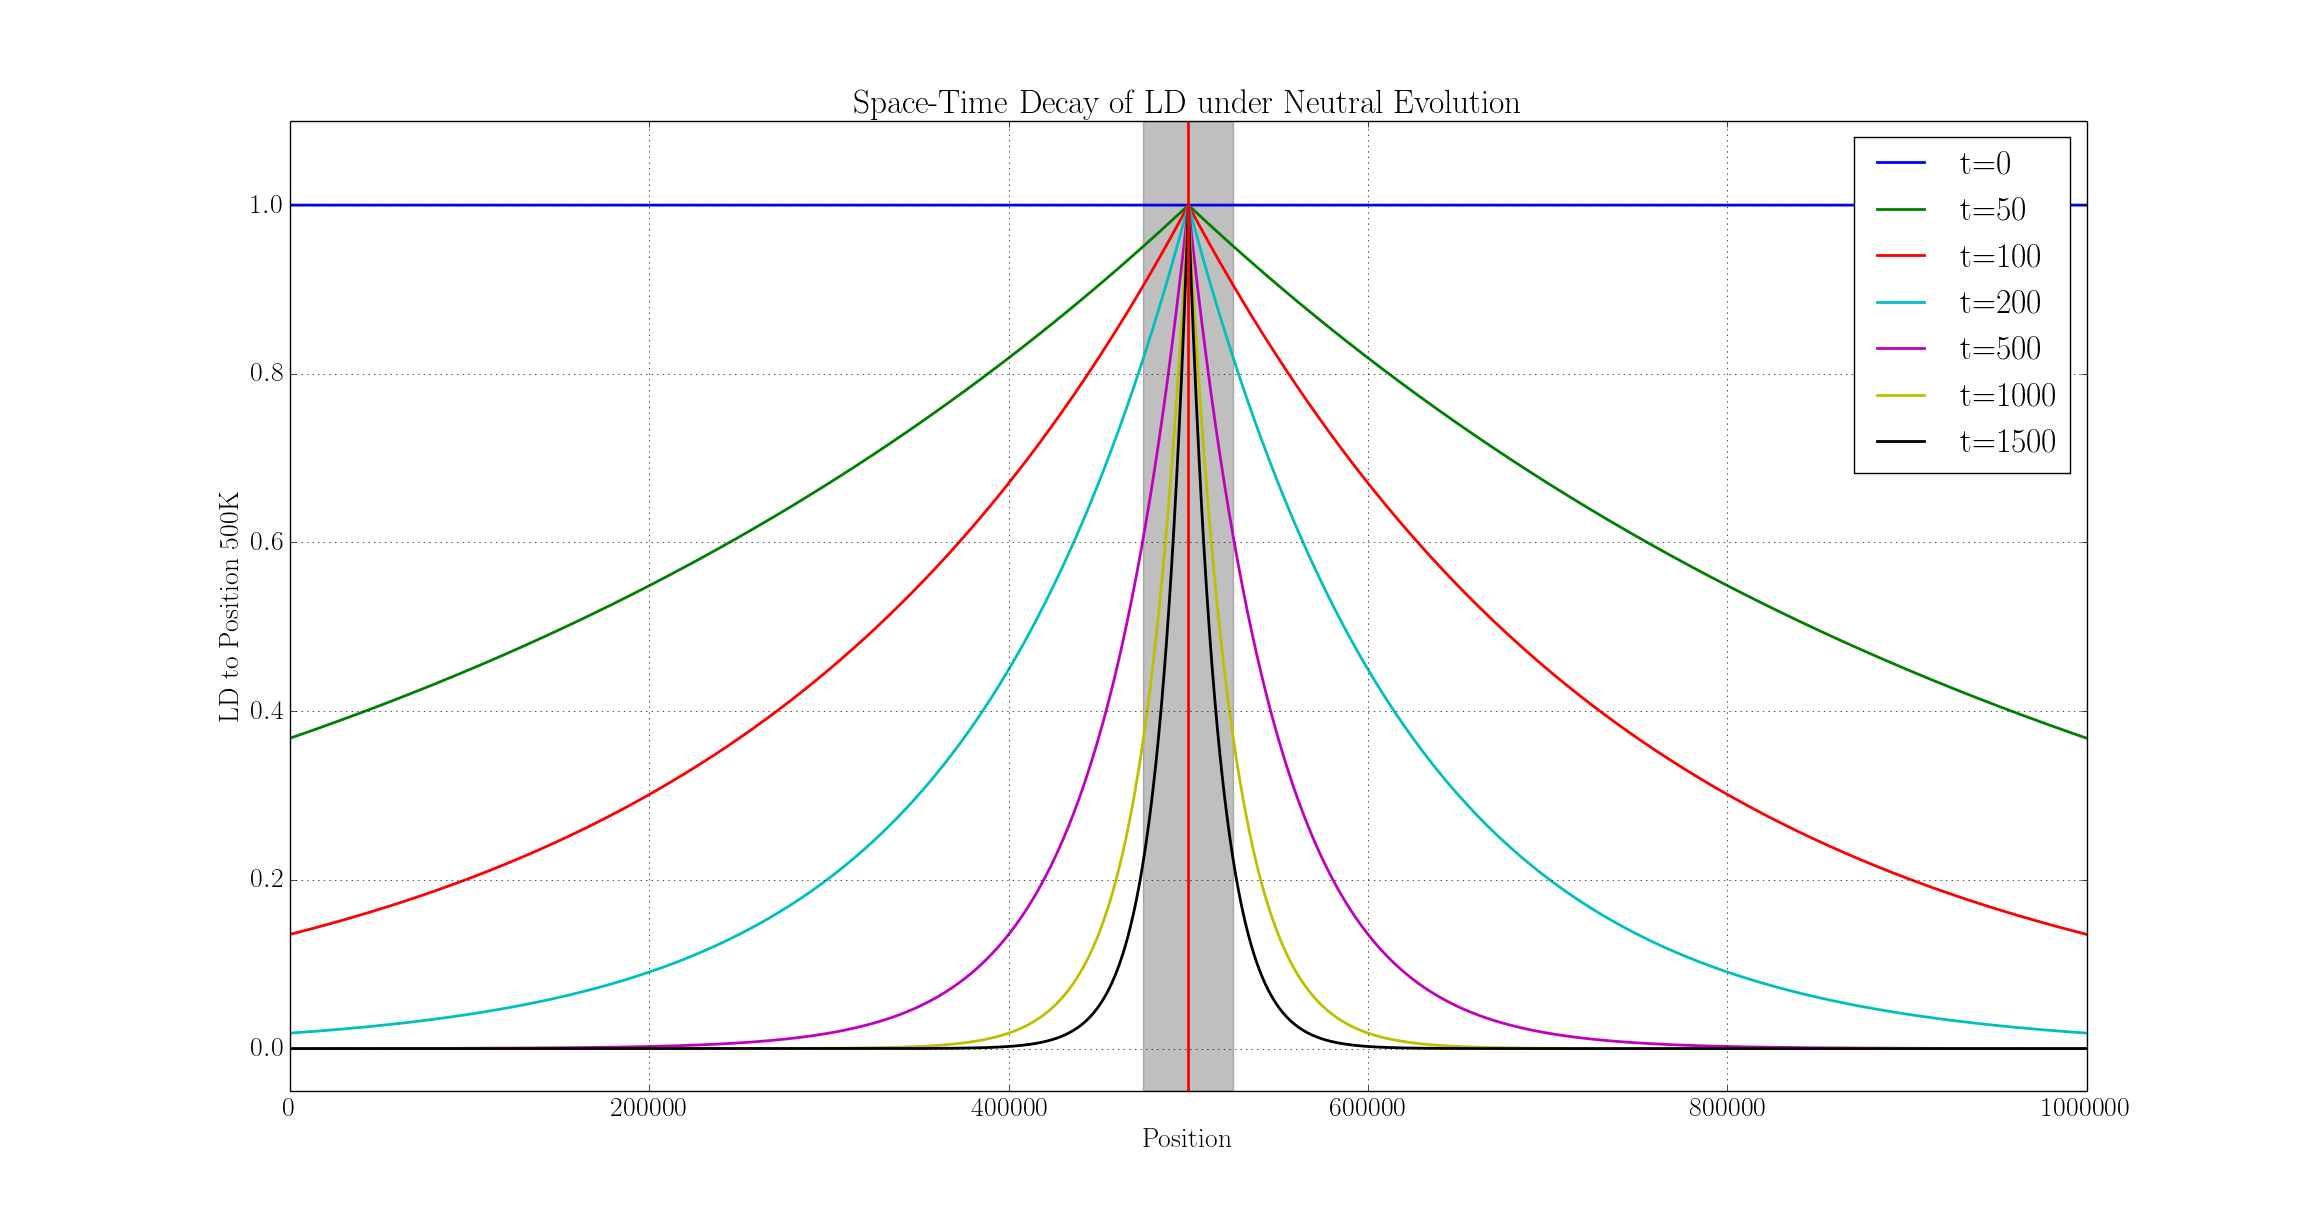
\includegraphics[scale=0.17]{spaceTimeLD}
\caption{Decay of LD in space through time under neutral evolution, when selected site is at position 500K. 50Kb window centered at the site is shaded.}

\end{figure}
\end{frame}

\begin{frame}{Multi Locus Model: Avg Haplotype Allele Frequency}
\begin{itemize}
\item Analogous to, TajimaD,H and SFSelect, AHAF is a statistic for a (50Kb) window can be computed instantly, (Euclidean norm of AF vector).
\item However, Ronen et. al. derived dynamics of AHAF in term of $\nu_t$ for hard sweep,  and therefore $s$.
\end{itemize}
\centering
\hspace{-0.1in}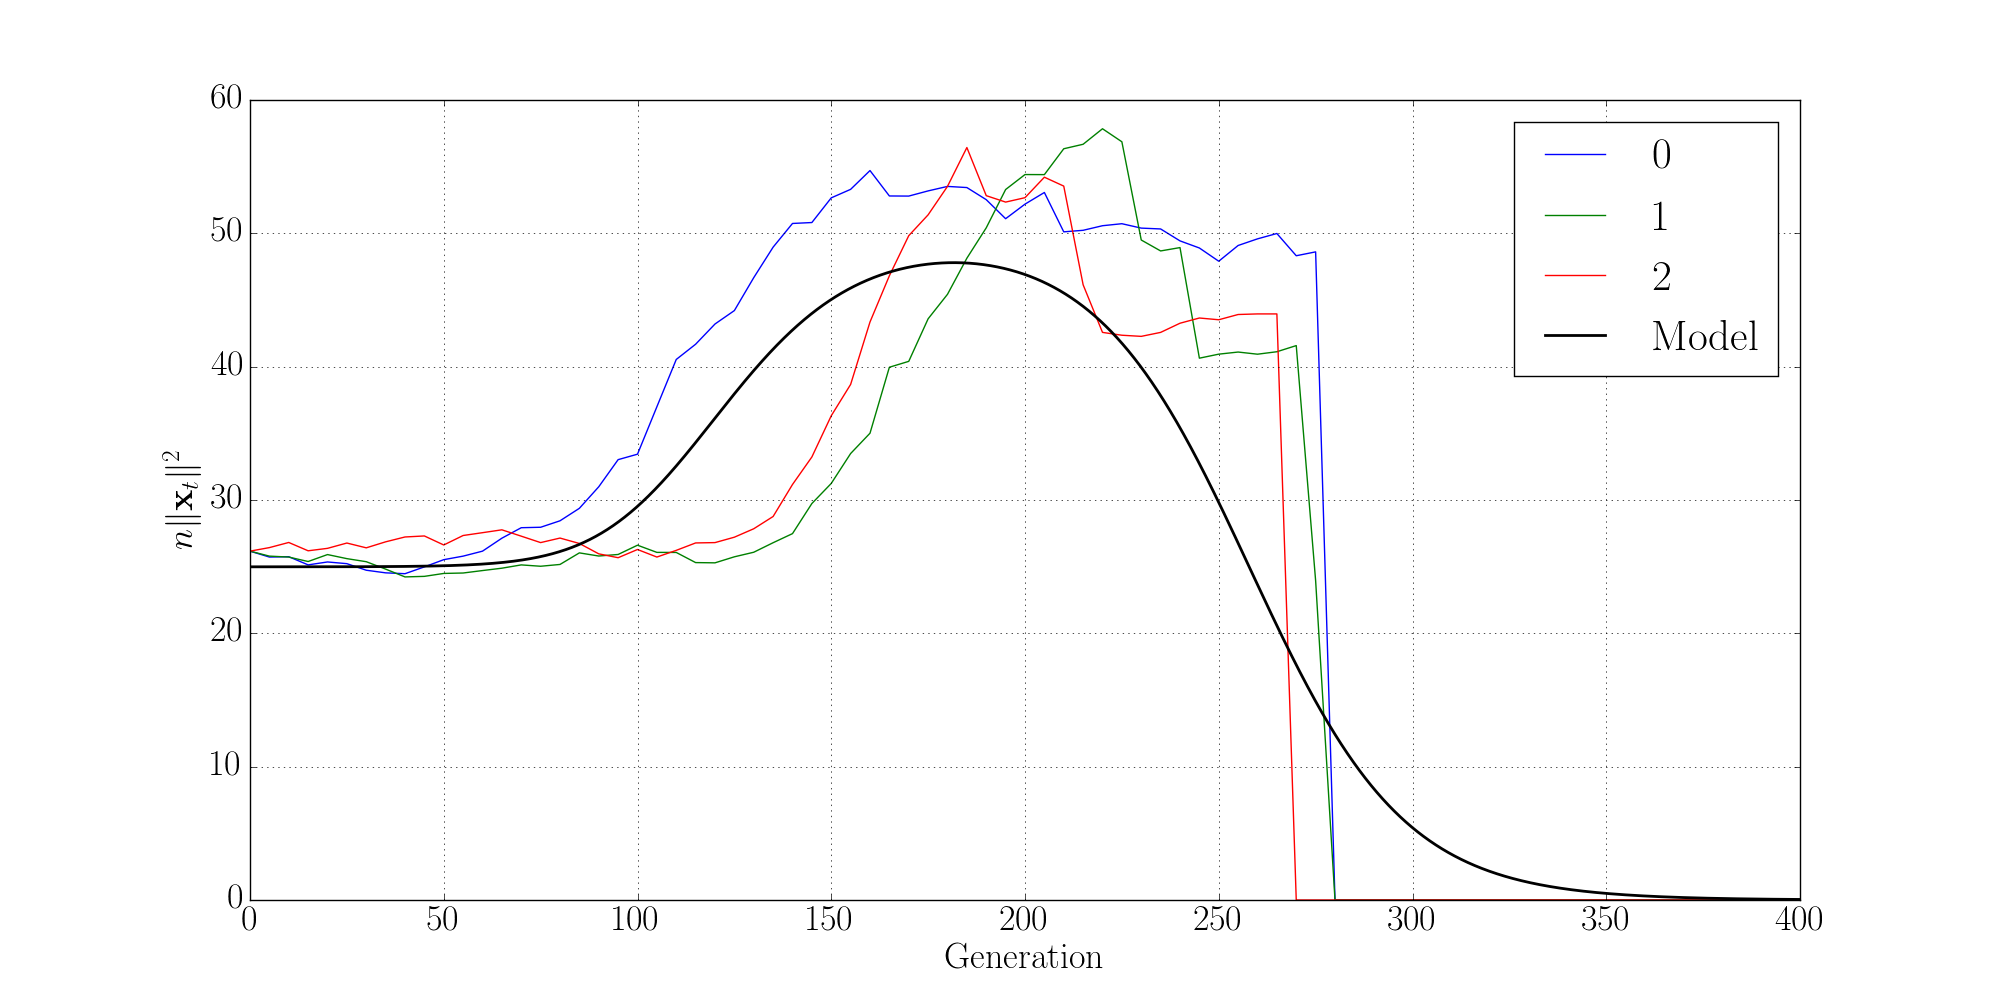
\includegraphics[scale=0.2]{haf}

\end{frame}



\begin{figure}
  \centering
  		    \includegraphics[trim={2in 0.5in 2in 0in},clip,width=\textwidth]{populationDynamics.pdf}
  \caption{A simulations for s=0.1. Mean of 10 replicates is shown as observation.
  Complete sweep is divided into three epochs based on carrier frequency.}
\end{figure}

\begin{frame}{Global Trends of sweep}
\begin{itemize}
\item In the following slides, global trend of Carrier freq, and all the window-based statistics are presented for each $s$.
\item There are two models: logistic (single locus) and AHAF (multi-locus).
\item 1000 simulations done and 95\% confidence interval is shown for each curve. (sweep/neutral).
\end{itemize}

\end{frame}

\begin{figure}[H]
  \centering
  		    \includegraphics[trim={2in 0.5in 2in 0in},clip,page=1,width=\textwidth]{Globaldynamics.pdf}
\end{figure}
{\tiny 1) Before generation 70, detection is difficult.\newline 2)Window based methods discriminate two cases with high confidence in phase 2 and 3.\newline 3) Discrimination in AHAF trend is harder than other methods.}

\begin{figure}[H]
  \centering
  		    \includegraphics[trim={2in 0.5in 2in 0in},clip,page=2,width=\textwidth]{Globaldynamics.pdf}
\end{figure}
{\tiny 1) Before generation 130, detection is difficult.\newline 2)Window based methods discriminate two cases with high confidence in phase 2 and 3.\newline 3) Discrimination in AHAF trend is harder than other methods.}

\begin{figure}[H]
  \centering
  		    \includegraphics[trim={2in 0.5in 2in 0in},clip,page=3,width=\textwidth]{Globaldynamics.pdf}
\end{figure}
{\tiny 1) Before generation 300, detection is difficult.\newline 2)Window based methods discriminate two cases with high confidence in phase 2 and 3.\newline 3) Discrimination in AHAF trend is harder than other methods.}


\begin{figure}[H]
  \centering
  		    \includegraphics[trim={2in 0.5in 2in 0in},clip,page=4,width=\textwidth]{Globaldynamics.pdf}
\end{figure}
{\tiny 1) Before generation 600, detection is difficult.\newline 2)Window based methods discriminate two cases with high confidence in phase 2 and 3.\newline 3) Discrimination in AHAF trend is harder than other methods.}

{\tiny Start of phases chosen when $\nu_t=[0.1,0.5,0.9]$ and AF sampled every 10 generations for 50 generations.}
\begin{figure}
\hspace{-0in}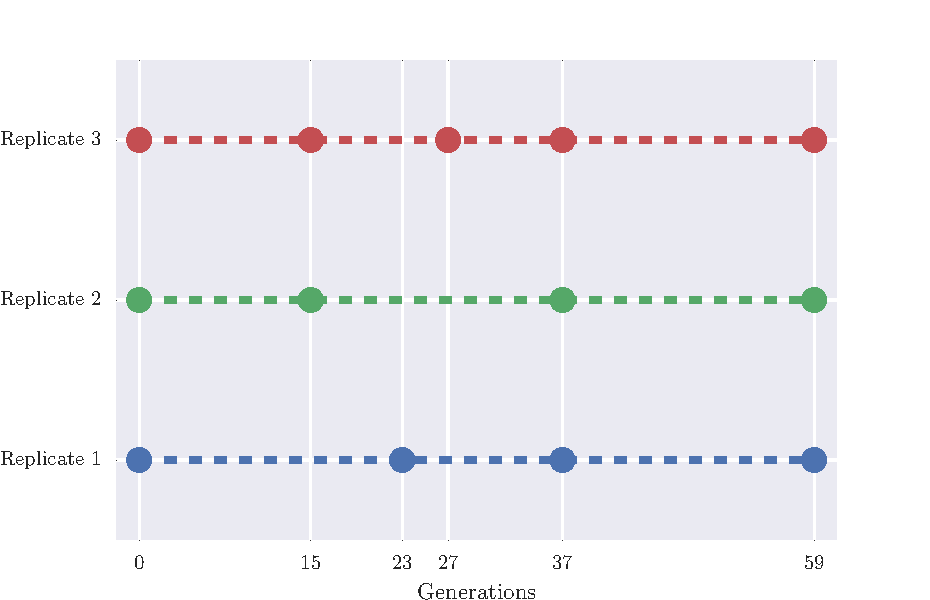
\includegraphics[scale=0.16]{samplingTimes}
\end{figure}
\vspace{-0.5in}



\begin{frame}{Task 1: Detecting Selection Experiments}
\begin{enumerate}[I]
\item To detect selection we need a predictor
\begin{itemize}
\item GP and HAF use Empirical Likelihood Ratio (ELR)
\beqq
ELR=\frac{Likelihood(Data|s=s^*)}{Likelihood(Data|s=0)}
\eeqq
\item Naive, use the ration of the first and last AF at a site
\item Model-free methods use their test-statistics values.
\end{itemize}
\item Single locus method (Naive and GP), use max of predictor over all the sites of the window.
\item performance measure is the percentage of Area under ROC curve, for regions with false-positive-rate is less than 0.1.
\end{enumerate}
\end{frame}



\begin{figure}[H]
  \centering
  		    \includegraphics[trim={0in 0.5in 0in 0in},clip,page=1,,scale=0.2]{aucfull}
\end{figure}
{\tiny \begin{enumerate}
\item Problem seems to be trivial if we have access to 5 time samples in a wide times series window (200,500,1000,2000 generations).
\item when $s$ is small, SFSelect outperforms the others.
\end{enumerate}}




\begin{figure}[H]
  \centering
  		    \includegraphics[trim={0in 0.5in 0in 0in},clip,page=1,,scale=0.2]{aucwin50.pdf}
\end{figure}
{\tiny \begin{enumerate}
\item Model-free methods perform very well in all epochs for sampling window = 50 , s=0.1.
\item Multi-locus methods are better than single locus ones.
\item Model-free methods are better than model-based ones.
\end{enumerate}}

\begin{figure}[H]
  \centering
  		    \includegraphics[trim={0in 0.5in 0in 0in},clip,page=2,scale=0.2]{aucwin50.pdf}
\end{figure}
{\tiny \begin{enumerate}
\item Model-free methods perform very well in last two epochs for sampling window = 50 , s=0.05.
\item Multi-locus methods are better than single locus ones.
\item Model-free methods are better than model-based ones.
\end{enumerate}}


\begin{figure}[H]
  \centering
  		    \includegraphics[trim={0in 0.5in 0in 0in},clip,page=3,,scale=0.2]{aucwin50.pdf}
\end{figure}
{\tiny \begin{enumerate}
\item Model-free methods perform very well in last two epochs for sampling window = 50 , s=0.02.
\item Multi-locus methods are better than single locus ones.
\item Model-free methods are better than model-based ones.
\end{enumerate}}


\begin{figure}[H]
  \centering
  		    \includegraphics[trim={0in 0.5in 0in 0in},clip,page=4,scale=0.2]{aucwin50.pdf}
\end{figure}
{\tiny \begin{enumerate}
\item Model-free methods perform very well in last two epochs for sampling window = 50 , s=0.01.
\item Multi-locus methods are better than single locus ones.
\item Model-free methods are better than model-based ones.
\end{enumerate}}


\begin{frame}{Task 2: Locating Selection}
Locating selection upto a 50Kb window amount to perform an sliding window detection test and select window with maximum predictor.
\end{frame}

\begin{frame}{Task 3: Estimating Strength Selection}
\begin{itemize}
\item Only model based method can estimate $s$.
\item Performance measure is absolute value of bias $|s-\hat{s}|$.
\end{itemize}
\end{frame}
\begin{figure}[H]
  \centering
  		    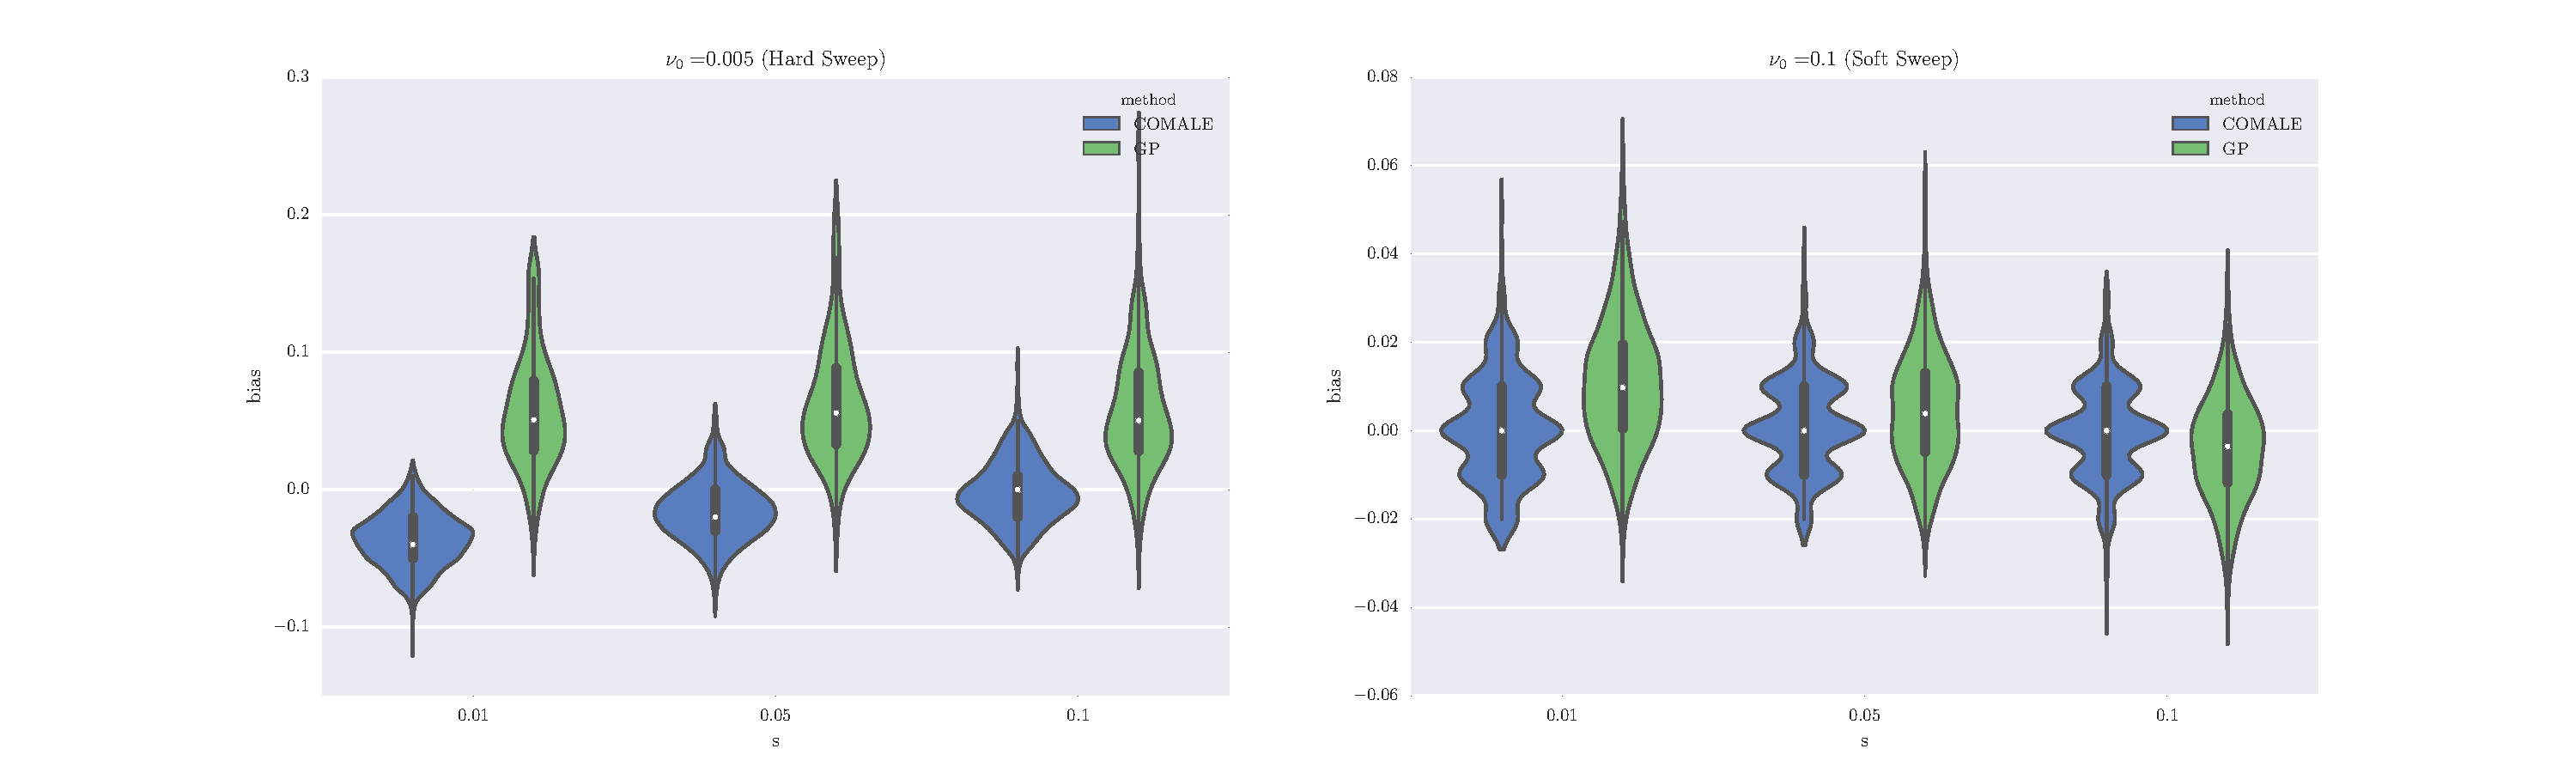
\includegraphics[trim={0in 0.5in 0in 0in},clip,page=1,,scale=0.2]{bias.pdf}
\end{figure}

\begin{figure}[H]
  \centering
  		    \includegraphics[trim={0in 0.5in 0in 0in},clip,page=2,,scale=0.2]{bias.pdf}
\end{figure}

\begin{figure}[H]
  \centering
  		    \includegraphics[trim={0in 0.5in 0in 0in},clip,page=3,,scale=0.2]{bias.pdf}
\end{figure}

\begin{figure}[H]
  \centering
  		    \includegraphics[trim={0in 0.5in 0in 0in},clip,page=4,,scale=0.2]{bias.pdf}
\end{figure}


\begin{frame}{summary}
\begin{itemize}
\item Classical model-free (multi-locus) methods work better for detecting and locating selection. 
\item HAF method is simple and its estimate of strength of selection is comparable to that of GP. However for detecting selection, HAF have too many FPs.
\item Verdict: Use classical model-free methods for detecting selection, if it exist, fit a HAF model to estimate $s$.
\item Sampling times are critical. In fact, given 5 samples along full sweep, the problem of detection is trivial.
\item To be verified: Due to high LD in experimental evolution in less than 2K generations, we can only determine window under selection, in HARD SWEEP.
\end{itemize}

\end{frame}


%\end{frame}


%
%\begin{frame}{Computational Performance}
%\begin{figure}[H]
%  \centering
%    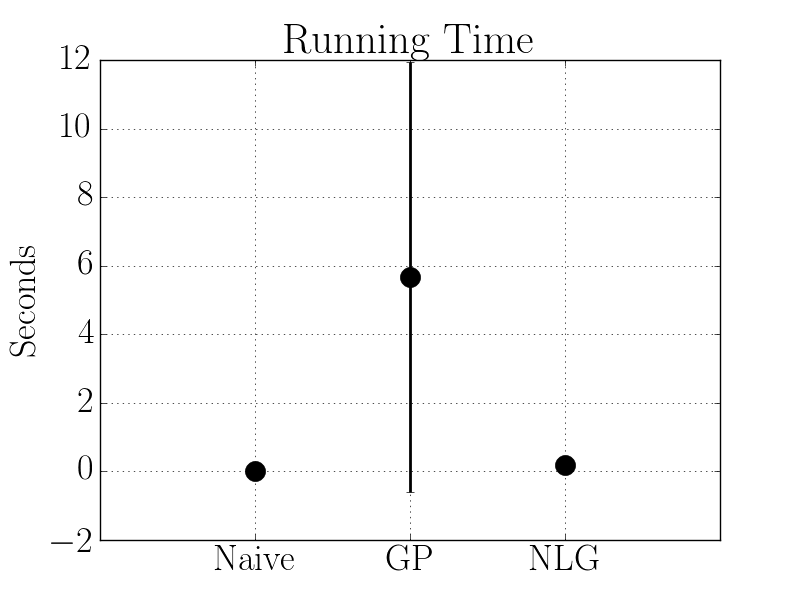
\includegraphics[width=0.6\textwidth]{times}
%\end{figure}
%\end{frame}





\begin{frame}{\ }
\vspace{1	in}
\begin{center}
	\huge{Thanks!}\\
\end{center}

\end{frame}

\begin{frame}{Single Locus Model: Carrier Frequency}
\begin{itemize}
\item By differentiating update equations ($x_{t+1}=x_t+\frac{sx_t(1-x_t)}{2+2sx_t}$ w.r.t. $t$ and solving differential equation, we have
\beqq
\nu_t=\sigma\left(st/2+\eta(\nu_0)\right)
\eeqq
where $\sigma(.)$ is logistic function and $\eta=\sigma^{-1}$ is the logit function and $\nu_t$ is the frequency of the carrier at time $t$.
\end{itemize}
\hspace{-0.6in}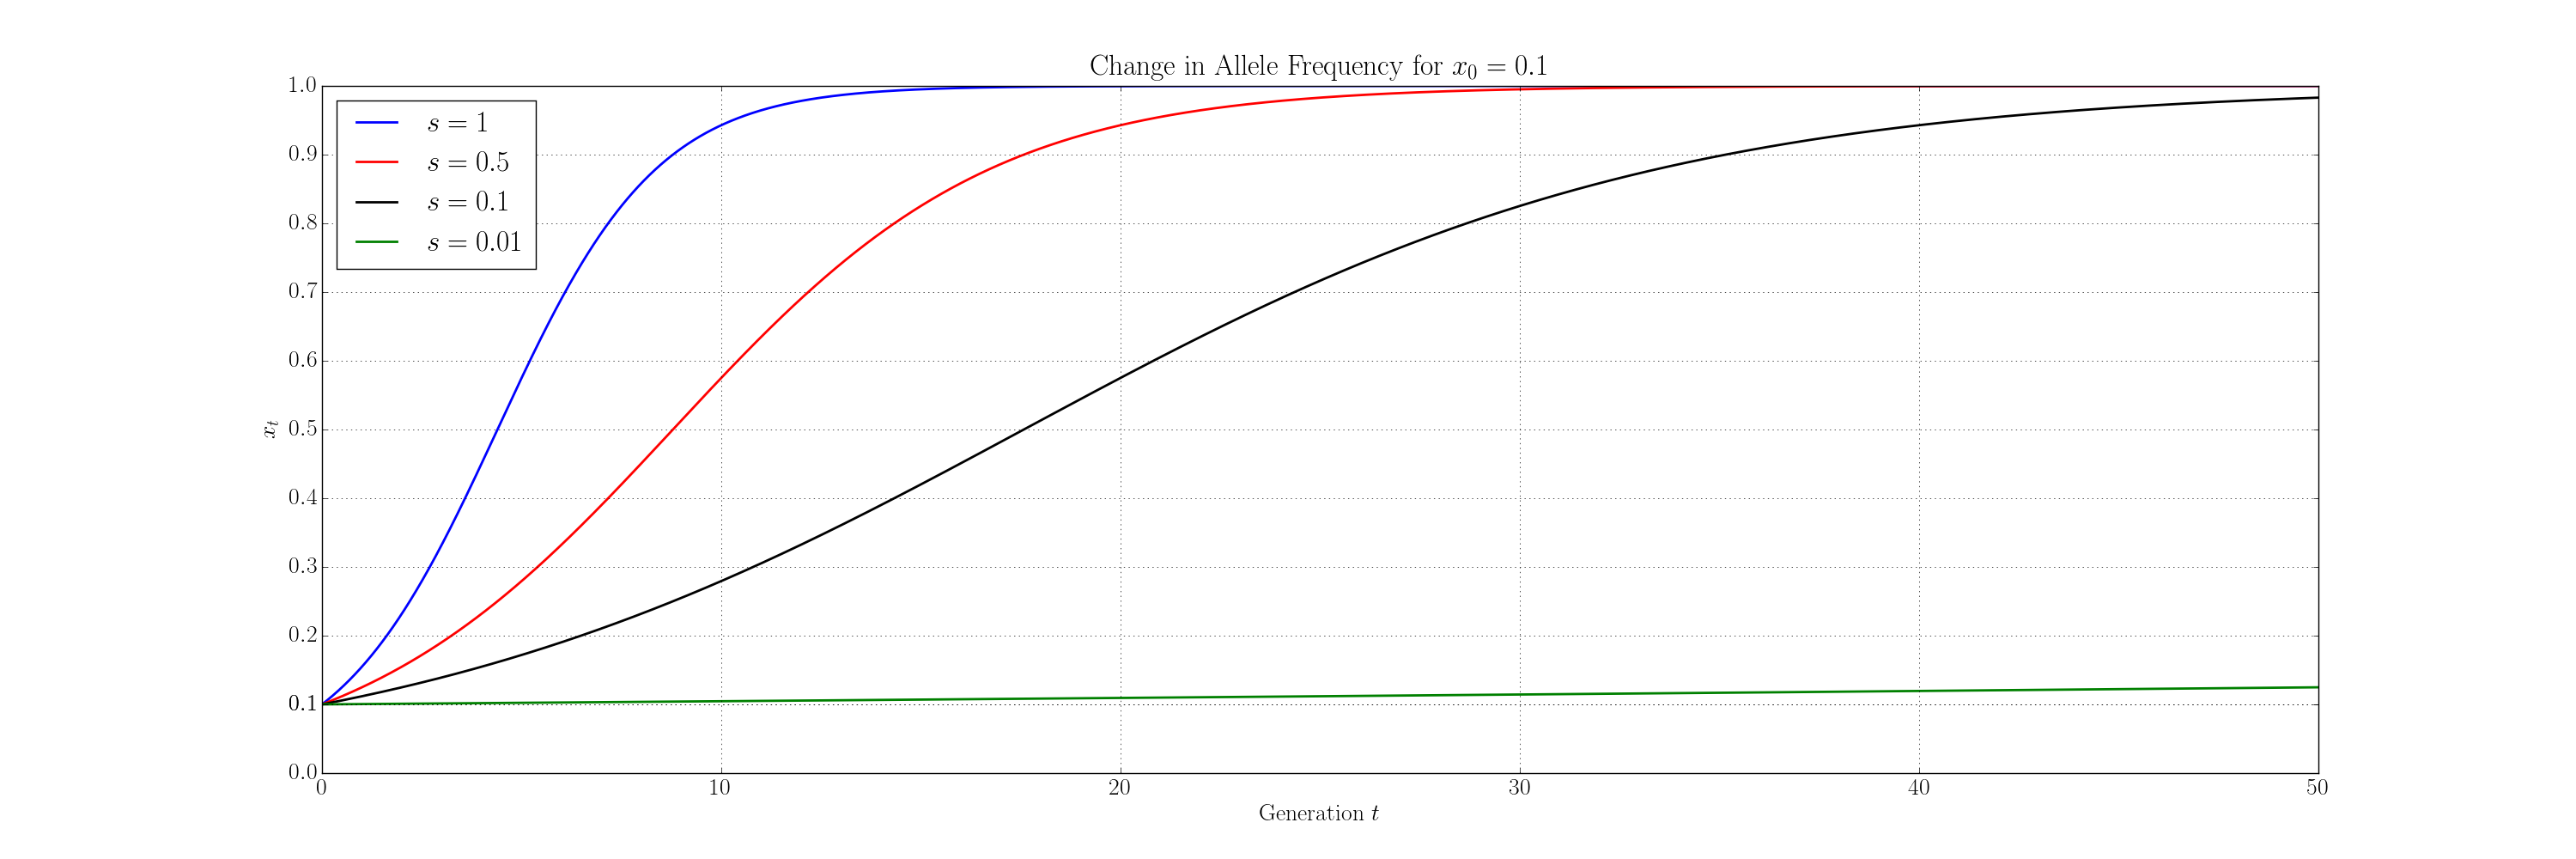
\includegraphics[scale=0.2]{sigmoid}
\end{frame}
\begin{frame}{Multi Locus Model: Average Haplotype Allele Frequency}

\begin{equation*}
\resizebox{.99\hsize}{!}{
$\mathbb{E}[1\dHAF(t)]= \|\mathbf{x}_t\|^2\approx \theta \nu_t \left(\frac{\nu_t+1}{2} - \frac{1}{(1-\nu_t)n+1}\right) +
 \theta (1-\nu_t)\left(\frac{n+1}{2n}-\frac{1}{(1-\nu_t)n+1}\right)$
}
\end{equation*}
where $ \mathbf{x}_t$ is vector of AF at time $t$ and $\nu_t=\sigma\left(st/2+\eta(\nu_0)\right)$.

\hspace{-0.1in}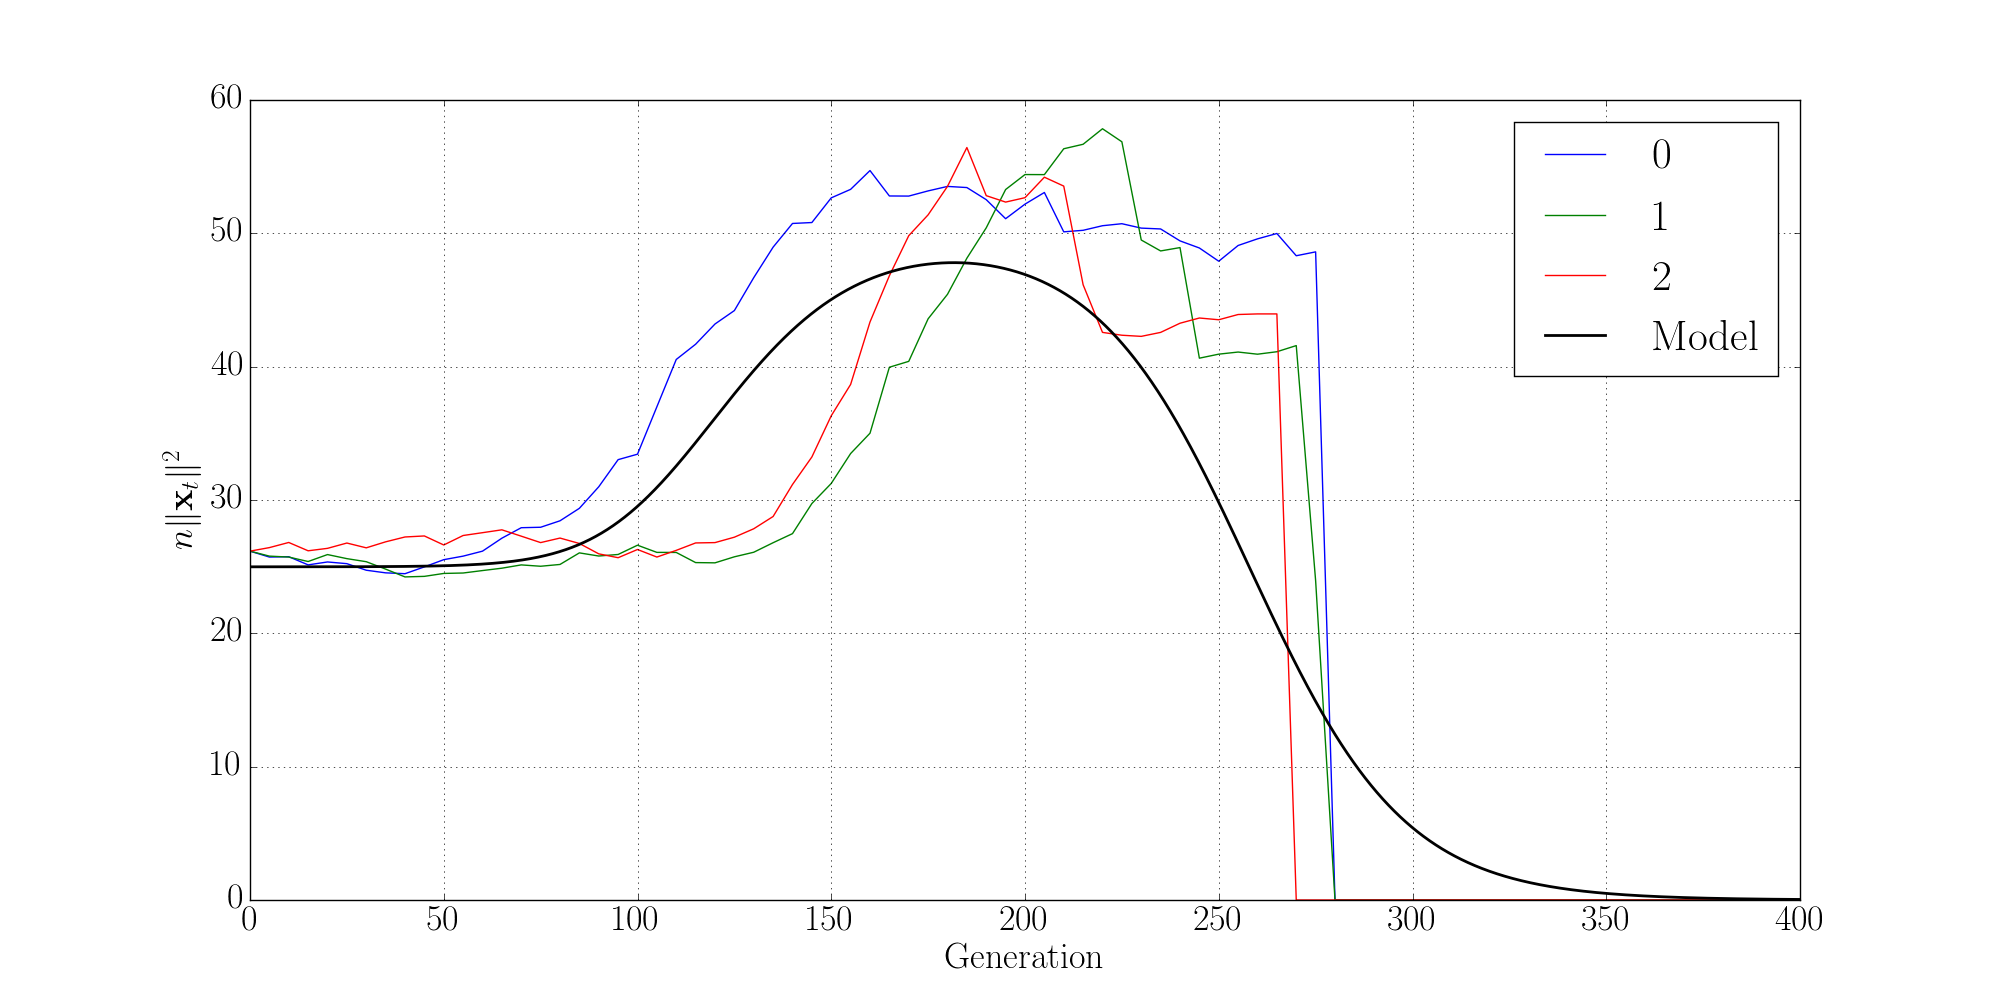
\includegraphics[scale=0.2]{haf}
\end{frame}
\begin{frame}{Critics to GP}
\begin{itemize}
\item Its too complex, likely to overfit with small number of iid replicates.
\item Although the likelihood model is based on different parameters, in practice, it can learn only one parameter at a time.
\item not tractable, its time complexity is quartic!
\item worse, each iteration requires \texttt{maxGeneration} recursion which makes it very hard to analyse late epochs of sweeps.
\item In addition to PoolSeq data, it requires initial population haplotypes.
\item Despite its elegant theory, it has not compared with classical methods.
\item In practice, single locus scan is performed and multi-locus (with 3-7 seg. sites.) model is fitted at regions of interests.
\end{itemize}
\end{frame}
\end{document}


